\subsection{Newton’s Geometry of Force: Kepler’s Second Law and the Birth of Gravity}

Building on his concept of \textit{fluxions}, Newton sought to explain the celestial mechanics that Kepler had described — particularly the Second Law: that a planet sweeps out equal areas in equal intervals of time.

But for Newton, this was more than an empirical fact — it was a geometric key.

\paragraph{Tangents and Areas.} Newton imagined a planet tracing a polygonal path around the sun, changing direction at small but finite intervals. The motion between each point was along a straight line — the tangent to the curve at that instant. A central force, acting in discrete impulses, would “bend” the path at each vertex toward the sun.

This construction allowed him to prove that if a body is always deflected toward a central point (like the Sun), then the areas swept out by its radius vector are equal over equal times.

\begin{figure}[H]
\centering
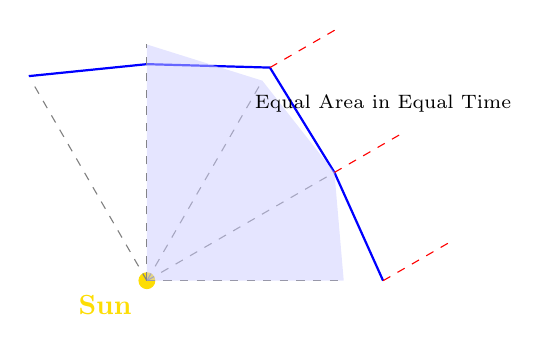
\begin{tikzpicture}[scale=2.5]

  % Sun at origin
  \filldraw[yellow!80!orange] (0,0) circle (0.04) node[below left=2pt] {\textbf{Sun}};

  % Orbit path (approx polygonal)
  \draw[thick, blue] (0:1.2) -- (30:1.1) -- (60:1.25) -- (90:1.1) -- (120:1.2);

  % Radius vectors
  \foreach \a in {0,30,60,90,120} {
    \draw[gray, dashed] (0,0) -- (\a:{1 + 0.2*sin(\a)});
  }

  % Tangents
  \draw[dashed, red] (0:1.2) -- ++(30:0.4);
  \draw[dashed, red] (30:1.1) -- ++(30:0.4);
  \draw[dashed, red] (60:1.25) -- ++(30:0.4);

  % Area sectors (for visual)
  \foreach \a/\b in {0/30, 30/60, 60/90} {
    \fill[blue!20, opacity=0.5] (0,0) -- (\a:{1 + 0.2*sin(\a)}) -- (\b:{1 + 0.2*sin(\b)}) -- cycle;
  }

  \node at (1.2, 0.9) {\scriptsize Equal Area in Equal Time};

\end{tikzpicture}
\caption{Newton’s polygonal construction: a planet moving in equal time steps traces out equal areas. Each segment approximates a tangent; each deflection represents a central force impulse.}
\end{figure}

\paragraph{From Area to Force.} In Proposition I of the \textit{Principia}, Newton proved:  

\textit{“A body under a centripetal force sweeps out equal areas in equal times.”}

The converse is also true: if equal areas are swept in equal time, then the force must point toward the center. The notion of “force” is geometric. It’s the repeated deflection of the tangent line by an inward-pulling agent.

\paragraph{From Fluxions to Gravity.} Once Newton had this geometric foundation, he began to explore the nature of the force itself.

In Proposition XI of the \textit{Principia}, he showed that if a planet’s orbit is an ellipse and the force is centripetal, then the force must be inversely proportional to the square of the distance:

\[
F \propto \frac{1}{r^2}
\]

To derive this, Newton analyzed how the velocity (the fluxion of position) changes along the curve. Using geometry and proportions, he established that the acceleration required to maintain the elliptical orbit — which he related to curvature and tangents — must obey this inverse-square law.

This, combined with Kepler’s laws, gave the world its first universal law of gravitation.

\paragraph{Tangents as the Language of Force.} In Newton’s hands, the tangent was more than a line — it was a law. The fluxion $\dot{x}$ described the direction and speed of a moving point; the change of the tangent described acceleration; and acceleration, in Newton’s system, was nothing other than force.

\[
\text{Fluxion} \rightarrow \text{Tangent} \rightarrow \text{Change of Tangent} \rightarrow \text{Force}
\]

This wasn’t just a mathematical trick — it was a physical revolution.

In Book I of the \textit{Principia}, Newton defined \textit{centripetal force} as any force that continually draws a body toward a center, keeping it in a curved path. But unlike earlier thinkers who assumed circular motion or treated the force qualitatively, Newton made the force *quantitative*. Using his method of fluxions and geometric reasoning, he calculated the acceleration of a body moving along any curve, not just a circle.

First, he considered a body tracing out a curve over time. The velocity — or fluxion — at any instant is tangent to the path. But as the body moves, the direction of the tangent changes. Newton focused on that change — not just in magnitude, but in direction — and recognized it as acceleration.

He then showed that this acceleration always points toward the center of curvature of the path — and this is precisely what he defined as \textit{centripetal force}. In the case of uniform circular motion, he derived the now-familiar formula:

\[
F = \frac{mv^2}{r}
\]

But his true innovation was generalizing this result. By connecting the changing tangent (i.e., curvature) with force, Newton was able to prove that **planetary motion**, as described by Kepler’s laws, could only be explained if the force pulling planets toward the Sun followed an inverse-square law:

\[
F \propto \frac{1}{r^2}
\]

This was a profound leap: geometry became physics. Tangents, once abstract tools of shape and slope, became vectors of speed, change, and gravitational pull. Where Euclid assumed tangents existed, Newton derived them — and then used them to bind the heavens.

Thus, Kepler’s geometry became Newton’s physics — with the fluxion as the bridge.
\begin{figure}[H]
\centering
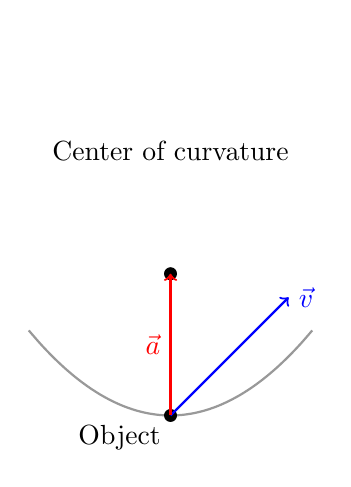
\begin{tikzpicture}[scale=1.5, 
    force/.style={->, thick, red}, 
    velocity/.style={->, thick, blue}, 
    path/.style={thick, black!40},
    point/.style={circle,fill=black,inner sep=1.5pt}]

% Draw curved path
\draw[path, domain=-1.2:1.2, smooth, variable=\t] 
    plot ({\t}, {0.5*\t*\t});

% Moving object
\coordinate (P) at (0,0); % point on curve
\filldraw[point] (P) circle (0.05);

% Tangent vector (velocity)
\draw[velocity] (P) -- ++(1,1) node[anchor=west] {$\vec{v}$};

% Radius to center of curvature (for a parabola, approximation)
\coordinate (C) at (0,1.2);
\draw[dashed] (C) -- (P);
\filldraw[point] (C) circle (0.05) node[above] {Center of curvature};

% Acceleration vector (normal to the curve, toward center)
\draw[force] (P) -- (C) node[midway,left] {$\vec{a}$};

% Label point
\node[below left] at (P) {Object};

\end{tikzpicture}
\caption{Newton’s insight: the change in the tangent vector (velocity) defines acceleration, which points toward the center — the direction of the centripetal force.}
\end{figure}





\subsubsection{Kepler’s Orbit, Newton’s Geometry: Aphelion and Perihelion in Motion}

Newton didn’t just prove that planetary motion obeys the equal-area rule — he used that geometry to explain how a planet accelerates as it nears the sun, and decelerates as it moves away. These critical points — known today as \textit{perihelion} (closest to the sun) and \textit{aphelion} (farthest from the sun) — are not locations with fixed speeds, but positions where velocity changes continuously. The reason lies in the geometry of swept areas and the evolving direction of motion.

\paragraph{Equal Areas, Unequal Speeds.}  
By Kepler’s second law, a planet sweeps out equal areas in equal times. But orbits are elliptical, not circular — so the radius changes constantly. Near perihelion, the radius is short; near aphelion, it's long. To keep the area swept out per unit time constant, the planet must move faster when closer to the sun, and slower when farther away.

Newton didn’t calculate this with algebra. He visualized it. He approximated the orbit as a polygon — a sequence of triangles, each swept out in equal intervals of time. In one step, the planet moves a short distance near the sun and a long distance when farther away. Yet the area of each triangle remains the same. The only way this can happen is if the speed increases as the radius decreases.

Since the area of a triangle is proportional to the product of the radius and the component of motion perpendicular to it, and since the areas are constant, Newton concluded:
\[
r \cdot v_\perp = \text{constant}
\]
Thus, when $r$ is small, the perpendicular velocity must be large — and vice versa.

No trigonometry was required. Just ratios, diagrams, and an unshakable commitment to geometric reasoning.

\paragraph{Tangents and the Geometry of Acceleration.}  
Newton took this one step further. He imagined the planet’s path as a sequence of infinitesimally short straight lines — tangents — continuously deflected by a central force. The force does not act along the tangent but perpendicular to it, pulling the planet inward.

The change in the tangent vector encodes acceleration:  
\[
\vec{a} = \frac{d\vec{v}}{dt}
\]
And because the direction of acceleration always points toward the sun, Newton concluded that **a central force** was at work.

But then, by measuring how quickly the direction of the tangent turns — and how far the planet moves along the curve — Newton showed that the magnitude of this acceleration decreases with the square of the distance:
\[
\vec{F} = m \vec{a} \propto \frac{1}{r^2}
\]

So from Kepler’s simple area law, Newton extracted a force law:
\[
\text{Equal Areas} \Rightarrow \text{Central Force} \Rightarrow \text{Inverse Square Law}
\]

This wasn’t algebraic deduction. It was geometry in motion: triangles in orbit, tangents that twist, and vectors that tell the story of gravity — not as a mystical pull, but as the logical consequence of space, motion, and time.

\begin{figure}[H]
\centering
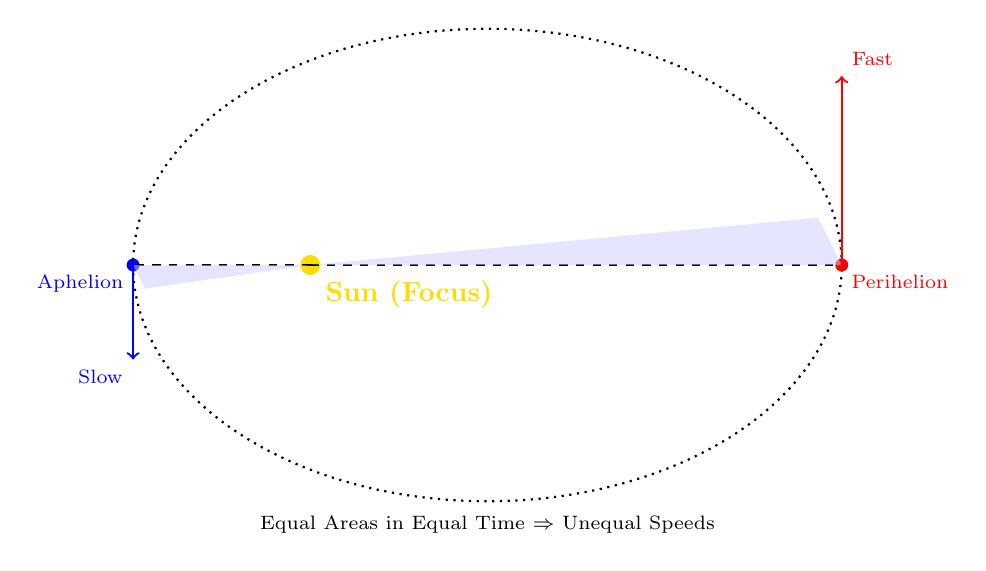
\begin{tikzpicture}[scale=3]

  % Elliptical orbit
  \draw[dotted, thick] (0,0) ellipse (1.5 and 1);

  % Sun at one focus
  \filldraw[yellow!80!orange] (-0.75,0) circle (0.04) node[below right=2pt] {\textbf{Sun (Focus)}};

  % Perihelion and Aphelion points
  \filldraw[red] (1.5,0) circle (0.025) node[below right] {\scriptsize Perihelion};
  \filldraw[blue] (-1.5,0) circle (0.025) node[below left] {\scriptsize Aphelion};

  % Radius vectors
  \draw[dashed, thick] (-0.75,0) -- (1.5,0);     % perihelion radius
  \draw[dashed, thick] (-0.75,0) -- (-1.5,0);    % aphelion radius

  % Corrected Equal-area wedges:
  % Perihelion: short radius, wide angle
  \fill[blue!20, opacity=0.5] (-0.75,0) -- (1.5,0) -- (1.4,0.2) -- cycle;

  % Aphelion: long radius, narrow angle
  \fill[blue!20, opacity=0.5] (-0.75,0) -- (-1.5,0) -- (-1.45,-0.1) -- cycle;

  % Corrected Tangents at perihelion and aphelion
  \draw[->, thick, red] (1.5,0) -- (1.5,0.8) node[above right] {\scriptsize Fast};
  \draw[->, thick, blue] (-1.5,0) -- (-1.5,-0.4) node[below left] {\scriptsize Slow};

  % Annotation
  \node[align=center] at (0,-1.1) {\scriptsize Equal Areas in Equal Time $\Rightarrow$ Unequal Speeds};

\end{tikzpicture}
\caption{Corrected geometry: Near perihelion (right), the radius is short, so the planet must move quickly, sweeping a short-wide wedge. Near aphelion (left), the radius is long, so the planet moves slowly, sweeping a long-narrow wedge. Newton derived these dynamics from geometry, not from formulas.}
\end{figure}


\paragraph{Geometry First, Numbers Later.}  
In Newton’s hands, physics began as a geometry problem. Only later would algebra catch up. The variation in orbital speed — now derivable from calculus — was, for Newton, embedded in the shape of triangles, the sweep of sectors, and the deflection of tangents.

The laws of the heavens were not equations on paper.  
They were drawn with straightedges, animated by force, and carved into orbits by geometry.



\begin{tcolorbox}[colback=blue!5!white, colframe=blue!50!black, 
  title={Historical Sidebar: Descartes—The Philosopher Newton Couldn't Ignore}]
  
      \textbf{René Descartes} (1596–1650) was the philosopher-scientist who set the stage for the entire Enlightenment—and unintentionally lit a fire under Newton. While Newton had little love for Descartes personally (he called his theories “fictions”), he couldn’t escape his influence. Descartes’ work was the scaffolding Newton climbed to build modern physics.
  
      \medskip
  
      Descartes viewed the universe as a giant geometric machine, governed by motion and mathematical rules. He invented \textbf{analytic geometry}—the system of coordinates and equations that made it possible to describe curves with algebra. Without it, there’s no framework for Newton’s calculus. No variables, no limits, no fluxions.
  
      \medskip
  
      Even Newton’s decision to frame calculus geometrically, rather than purely algebraically like Leibniz, owes something to Descartes’ method of using shapes to describe motion. And though Newton eventually rejected Descartes’ physics—especially his vortex theory—he kept Descartes’ core belief: that nature could be \textbf{understood through math, modeled by geometry, and predicted through logic}.
  
      \medskip
  
      \textbf{Quote from Descartes (1637):}
      \begin{quote}
      “Give me extension and motion, and I will construct the universe.”
      \end{quote}
  
      Newton gave him both—and added gravity. Even when he disagreed, \textbf{Newton never stopped arguing with Descartes}. Which, in philosophy, is just another form of admiration.
  
\end{tcolorbox}













